%%%%%%%%%%%%%%%%%%%%%%%%%%%%%%%%%%%%%%%%%%%%%%%%%%%%%%%%%%%%%%%%%%%%%
%%                                                                 %%
%% Please do not use \input{...} to include other tex files.       %%
%% Submit your LaTeX manuscript as one .tex document.              %%
%%                                                                 %%
%% All additional figures and files should be attached             %%
%% separately and not embedded in the \TeX\ document itself.       %%
%%                                                                 %%
%%%%%%%%%%%%%%%%%%%%%%%%%%%%%%%%%%%%%%%%%%%%%%%%%%%%%%%%%%%%%%%%%%%%%

%%\documentclass[referee,sn-basic]{sn-jnl}% referee option is meant for double line spacing

%%=======================================================%%
%% to print line numbers in the margin use lineno option %%
%%=======================================================%%

%%\documentclass[lineno,sn-basic]{sn-jnl}% Basic Springer Nature Reference Style/Chemistry Reference Style

%%======================================================%%
%% to compile with pdflatex/xelatex use pdflatex option %%
%%======================================================%%

%%\documentclass[pdflatex,sn-basic]{sn-jnl}% Basic Springer Nature Reference Style/Chemistry Reference Style

%%\documentclass[sn-basic]{sn-jnl}% Basic Springer Nature Reference Style/Chemistry Reference Style
\documentclass[pdflatex,sn-mathphys]{sn-jnl}% Math and Physical Sciences Reference Style
%%\documentclass[sn-aps]{sn-jnl}% American Physical Society (APS) Reference Style
%%\documentclass[sn-vancouver]{sn-jnl}% Vancouver Reference Style
%%\documentclass[sn-apa]{sn-jnl}% APA Reference Style
%%\documentclass[sn-chicago]{sn-jnl}% Chicago-based Humanities Reference Style
%%\documentclass[sn-standardnature]{sn-jnl}% Standard Nature Portfolio Reference Style
%%\documentclass[default]{sn-jnl}% Default
%%\documentclass[default,iicol]{sn-jnl}% Default with double column layout

%%%% Standard Packages
%%<additional latex packages if required can be included here>
%%%%

%%%%%=============================================================================%%%%
%%%%  Remarks: This template is provided to aid authors with the preparation
%%%%  of original research articles intended for submission to journals published 
%%%%  by Springer Nature. The guidance has been prepared in partnership with 
%%%%  production teams to conform to Springer Nature technical requirements. 
%%%%  Editorial and presentation requirements differ among journal portfolios and 
%%%%  research disciplines. You may find sections in this template are irrelevant 
%%%%  to your work and are empowered to omit any such section if allowed by the 
%%%%  journal you intend to submit to. The submission guidelines and policies 
%%%%  of the journal take precedence. A detailed User Manual is available in the 
%%%%  template package for technical guidance.
%%%%%=============================================================================%%%%

\jyear{2022}%
\usepackage{xstring}
\usepackage{float}
%% as per the requirement new theorem styles can be included as shown below
\theoremstyle{thmstyleone}%
\newtheorem{theorem}{Theorem}%  meant for continuous numbers
%%\newtheorem{theorem}{Theorem}[section]% meant for sectionwise numbers
%% optional argument [theorem] produces theorem numbering sequence instead of independent numbers for Proposition
\newtheorem{proposition}[theorem]{Proposition}% 
%%\newtheorem{proposition}{Proposition}% to get separate numbers for theorem and proposition etc.

\theoremstyle{thmstyletwo}%
\newtheorem{example}{Example}%
\newtheorem{remark}{Remark}%
\newcommand{\betterref}[1]{\IfBeginWith{#1}{fig:}{Fig.~}{Table~}\ref{#1}}
\theoremstyle{thmstylethree}%
\newtheorem{definition}{Definition}%

\raggedbottom
%%\unnumbered% uncomment this for unnumbered level heads

\begin{document}

\title[Analysis of PBMC Gene Expression Data in Asthmatic Patients]{Analysis of PBMC Gene Expression Data in Asthmatic Patients}

%%=============================================================%%
%% Prefix	-> \pfx{Dr}
%% GivenName	-> \fnm{Joergen W.}
%% Particle	-> \spfx{van der} -> surname prefix
%% FamilyName	-> \sur{Ploeg}
%% Suffix	-> \sfx{IV}
%% NatureName	-> \tanm{Poet Laureate} -> Title after name
%% Degrees	-> \dgr{MSc, PhD}
%% \author*[1,2]{\pfx{Dr} \fnm{Joergen W.} \spfx{van der} \sur{Ploeg} \sfx{IV} \tanm{Poet Laureate} 
%%                 \dgr{MSc, PhD}}\email{iauthor@gmail.com}
%%=============================================================%%

\author{\fnm{Kieran} \sur{Ford}}\email{kieran.ford@ufl.edu}

\author{\fnm{Richard} \sur{Garber}}\email{richard.garber@ufl.edu}

\author{\fnm{Jonathan} \sur{Kahn}}\email{jonathan.kahn@ufl.edu}


%%==================================%%
%% sample for unstructured abstract %%
%%==================================%%

\abstract{Asthma is a very common inflammatory disease affecting the lungs and reducing the quality of life of those who suffer it. Previous studies state that there is broad variability to how asthma presents itself throughout a sufferer’s lifetime \cite{Holgate2015-oz}. There are suggestions in previous research that asthma acquisition may be linked with altered immune system pathways \cite{Camiolo2021-gh, Holgate2015-oz, Holgate2012-et}, Previous studies have identified 73 differentially expressed genes compared between asthmatic and non-asthmatic patients \cite{Cao2022-im}. However, these studies have not looked to identify a link specifically between the differentially expressed genes (DEGs) and the expression of cells of the immune system. In this study, we analyzed NGS data from peripheral blood mononuclear cells (PBMCs) among a group of 42 patients with asthma and 14 patients without asthma to identify any statistically significant differentially expressed genes (SSDEGs) and to conduct enrichment analysis and unsupervised clustering analysis to identify a link between the expression in the immune cells and asthma acquisition. Here we identify 65 DEGs but fail to find any SSDEGs. Enrichment analysis on the DEGs identified links to the biological processes of responses to fungus and other stimuli. This may suggest a link between the expression in the immune cells and asthma acquisition. Additionally, clustering analysis suggested no clear link between the expression of the immune cells and asthma acquisition. We expect our varying findings to act as a starting point for additional research into SSDEGs in immune cells relating to asthma acquisition and severity. Further experimentation with larger sample sizes will be required to further investigate links with a greater possibility of statistical significance.}

%%================================%%
%% Sample for structured abstract %%
%%================================%%

% \abstract{\textbf{Purpose:} The abstract serves both as a general introduction to the topic and as a brief, non-technical summary of the main results and their implications. The abstract must not include subheadings (unless expressly permitted in the journal's Instructions to Authors), equations or citations. As a guide the abstract should not exceed 200 words. Most journals do not set a hard limit however authors are advised to check the author instructions for the journal they are submitting to.
% 
% \textbf{Methods:} The abstract serves both as a general introduction to the topic and as a brief, non-technical summary of the main results and their implications. The abstract must not include subheadings (unless expressly permitted in the journal's Instructions to Authors), equations or citations. As a guide the abstract should not exceed 200 words. Most journals do not set a hard limit however authors are advised to check the author instructions for the journal they are submitting to.
% 
% \textbf{Results:} The abstract serves both as a general introduction to the topic and as a brief, non-technical summary of the main results and their implications. The abstract must not include subheadings (unless expressly permitted in the journal's Instructions to Authors), equations or citations. As a guide the abstract should not exceed 200 words. Most journals do not set a hard limit however authors are advised to check the author instructions for the journal they are submitting to.
% 
% \textbf{Conclusion:} The abstract serves both as a general introduction to the topic and as a brief, non-technical summary of the main results and their implications. The abstract must not include subheadings (unless expressly permitted in the journal's Instructions to Authors), equations or citations. As a guide the abstract should not exceed 200 words. Most journals do not set a hard limit however authors are advised to check the author instructions for the journal they are submitting to.}


%%\pacs[JEL Classification]{D8, H51}

%%\pacs[MSC Classification]{35A01, 65L10, 65L12, 65L20, 65L70}

\maketitle

\section{Introduction}\label{sec1}

Asthma affects greater than 300 million individuals which is predicted to increase as more countries around the world adopt lifestyles similar to developed western countries \cite{Holgate2015-oz}. There are many suggestions about what causes asthma to develop in humans and at what stage. Some previous studies have identified certain immune responses to fungus as having an association with asthma severity as well as a possible relationship to inflammation in pathways with helper T cells \cite{Denning2006-jd, Holgate2012-et}. Other genome-wide association studies (GWAS) also identified differentially expressed genes in asthma patients and loci of interest in the immune system \cite{Cao2022-im, Zhu2018-zh}. In this study we focused on supporting these suggestions and findings of possible links between immune cells and asthma acquisition by focusing on a more simplified level of analysis. The research question we sought to answer was, What are the differences in gene expression within peripheral blood mononuclear cells between patients with moderate or severe asthma and healthy patients? To adequately answer this question, we used a next generation sequencing (NGS) counts dataset from the NCBI GEO database, GSE207751, which contained a total of 56 samples – 42 asthma patients and 14 patients without asthma. The samples came from PBMCs and the asthma patients had varying levels of severity identified in their metadata. The metadata also included other characteristics of the patients such as age and gender. The data was collected from peripheral blood mononuclear cells (PBMCs) which are cells with a round nucleus in the bloodstream, with most being lymphocytes and monocytes \cite{Pourahmad2015-dw}. These cells make up a large part of the immune system and T cells are a type of lymphocyte. Altered immune systems could be displayed via differentially expressed genes within this class of cells, which we can identify through our counts data and run through enrichment analysis to identify the pathways of these differentially expressed genes.
\section{Methods}\label{sec2}
All code can be found and the GitHub repository here: \href{https://github.com/rgarber11/GeGnomes-BioInformatics-Project}{https://github.com/rgarber11/GeGnomes-BioInformatics-Project} \\
Before analysis could be done using the data set, there was some formatting that needed to be done. The data set identified genes by Ensembl ID, these needed to be replaced with HGNC symbols, this was done using the \texttt{biomaRt} library in R \cite{Steffen_Durinck_biomartdevgmailcom_Wolfgang_Huber2017-mr}. The counts were then TPM normalized, and saved as fixed\_normalized\_counts.csv. A log-scaled and TPM normalized version was also created. \\
\texttt{DESeq2} was used to apply a VST and normalize data. This VST-normalized data was used to generate both the PCA plot and the assay data for M3C’s TSNE plot \cite{Love2014-fy, Zhu2019-jm,John2018-os}. All plots were also created using \texttt{ggplot2}. For differential expression a volcano plot was created using DESeq data and a pCutoff value of 0.01. A heatmap \cite{Gu2016-vz} was created using the log scaled counts data of genes that were found to be differentially expressed, with an annotation dividing samples into healthy and asthmatic groups.
Enrichment analysis on all genes with a logFoldChange greater than 1 is performed with the GO biological processes, the GO cellular components, and the REAC databases using the g:Profiler tool \cite{Raudvere2019-bp, ashburner2000gene, fabregat2018reactome}. \\
Clustering was performed three times on the dataset using three different methods: PAM clustering, K-means \cite{clusterpackage}, and \texttt{ConsensusClusterPlus} \cite{Wilkerson2010-aw}. To perform clustering an additional column was added to the counts data that contains variance and counts were ordered by variance. Finally the data was broken into smaller sets so clustering could be done with different amounts of genes. For each clustering method, different k values were tested, in the end PAM and K-means clustering was done with a k value of 2. Consensus clustering was done with a max K value of 20, the hierarchical clustering method, the Pearson method of determining distance, 1000 repetitions, and with 80\% of items sampled and 100\% of features sampled.  Sankey diagrams were created for each clustering method comparing the results of clustering with only 10, 100, 1000, 5000, and 10000 genes using the \texttt{ggalluvial} library \cite{ggalluvial-article}. The results of these clustering methods were used to annotate a heatmap \cite{Gu2016-vz} of the top five thousand genes by variance, showing which samples  The results of clustering were compared against each other and the original condition using a chi square test. They were then adjusted due to there being 6 different tests, and interpreted with a cutoff of $p > 0.05$.

\section{Results}\label{sec3}
Overall, we were unable to find a statistically significant difference in gene expression between people with or without asthma. While the dataset contained some variability as seen in Fig.~\ref{fig:density}, a PCA plot and t-SNE show that a majority of the variance does not come from whether participants had asthma, as seen in Figs.~\ref{fig:pca} and \ref{fig:tsne}.  Meanwhile, as can be seen in \betterref{tab:deseq}, DeSeq analysis shows that while certain singular tests would be independently significant, no test meets the barrier of $p < 0.5$ for statistical significance when taken together. That none of the genes expressed are significant can also be seen in Figs.~\ref{fig:volcano} and \ref{fig:heatmap}. Thus, while certain genes are differentially expressed, none meet the criterion to give an affirmative answer to the experimental question. \\
\begin{table}[H]
    \centering
    \resizebox{\textwidth}{!}{\begin{tabular}{@{}lllllll@{}}
    \toprule
        Gene & baseMean & log2FoldChange & lfcSE & pvalue & padj & threshold \\
\midrule
LRRC58-DT & 1.0412624 & 4.321867 & 1.4174352 & 4.371686e-02 & 0.4221497 & FALSE\\
MTND1P23 & 1.6782038 & 4.147562 & 1.2979116 & 3.610390e-02 & 0.3978533 & FALSE\\
ADAMTS2 & 13.4136189 & 3.982281 & 0.9256661 & 5.165539e-05 & 0.2052859 & FALSE\\
RPS20P13 & 0.6143606 & 3.710406 & 2.1985731 & 3.435173e-03 & 0.2504310 & FALSE\\
SLC6A19 & 16.7556055 & 3.536763 & 0.3928395 & 9.961202e-01 & 0.9994219 & FALSE\\
MTCO1P12 & 85.5174753 & 3.021756 & 0.5250292 & 8.666273e-03 & 0.2780836 & FALSE \\
\bottomrule
    \end{tabular}}
    \caption{DeSeq data showing statistical significance of the most differentially expressed genes.}
    \label{tab:deseq}
\end{table}
\begin{figure}[h!]
    \centering
    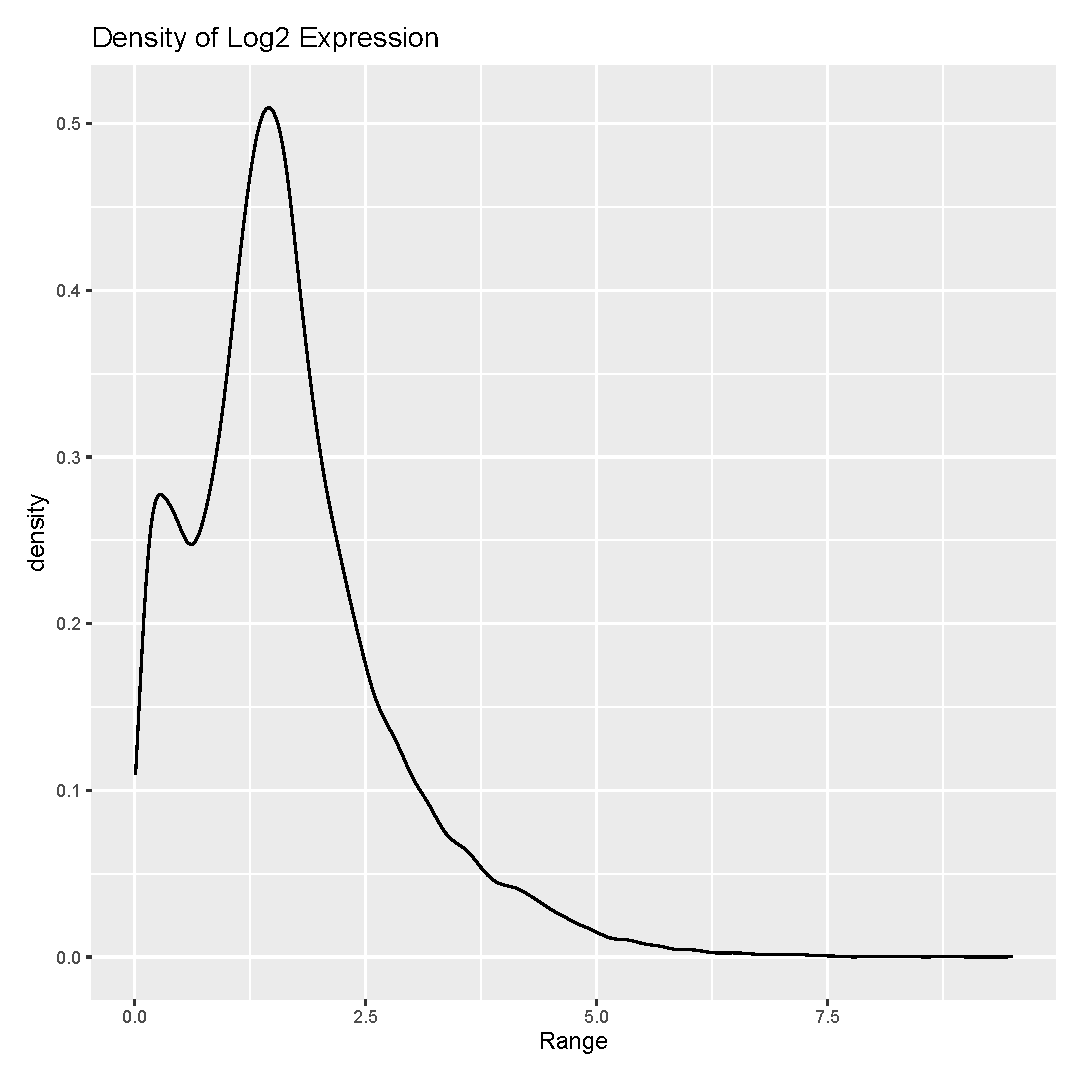
\includegraphics[scale=0.4]{plots/assn2/density_plot.eps}
    \caption{Log-Range Density of Gene Expression}
    \label{fig:density}
\end{figure}
\begin{figure}[h!]
    \centering
    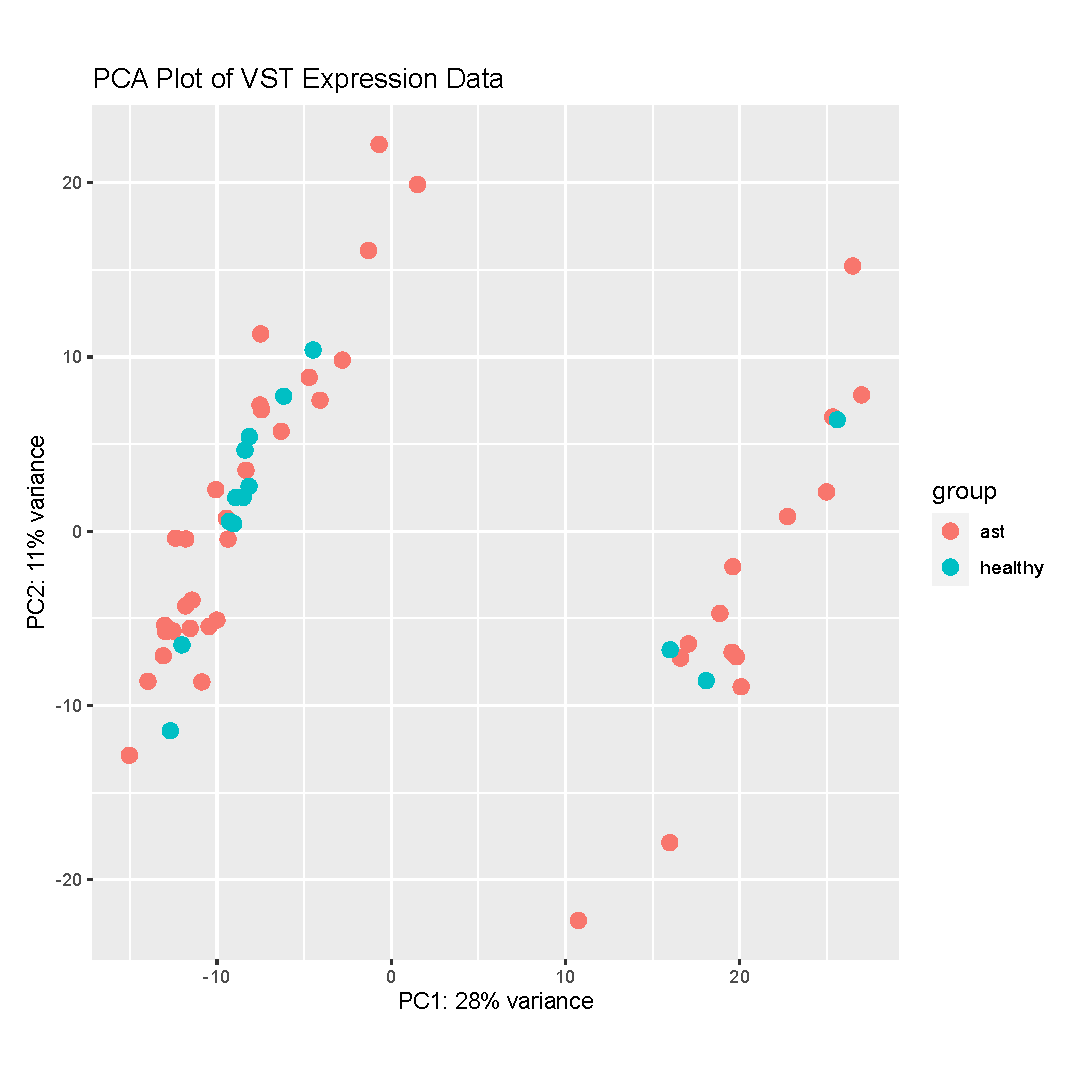
\includegraphics[scale=0.5]{plots/assn2/pca_plot.eps}
    \caption{PCA Plot of DeSeq of Gene Expression Data}
    \label{fig:pca}
\end{figure}
\begin{figure}[ht!]
    \centering
    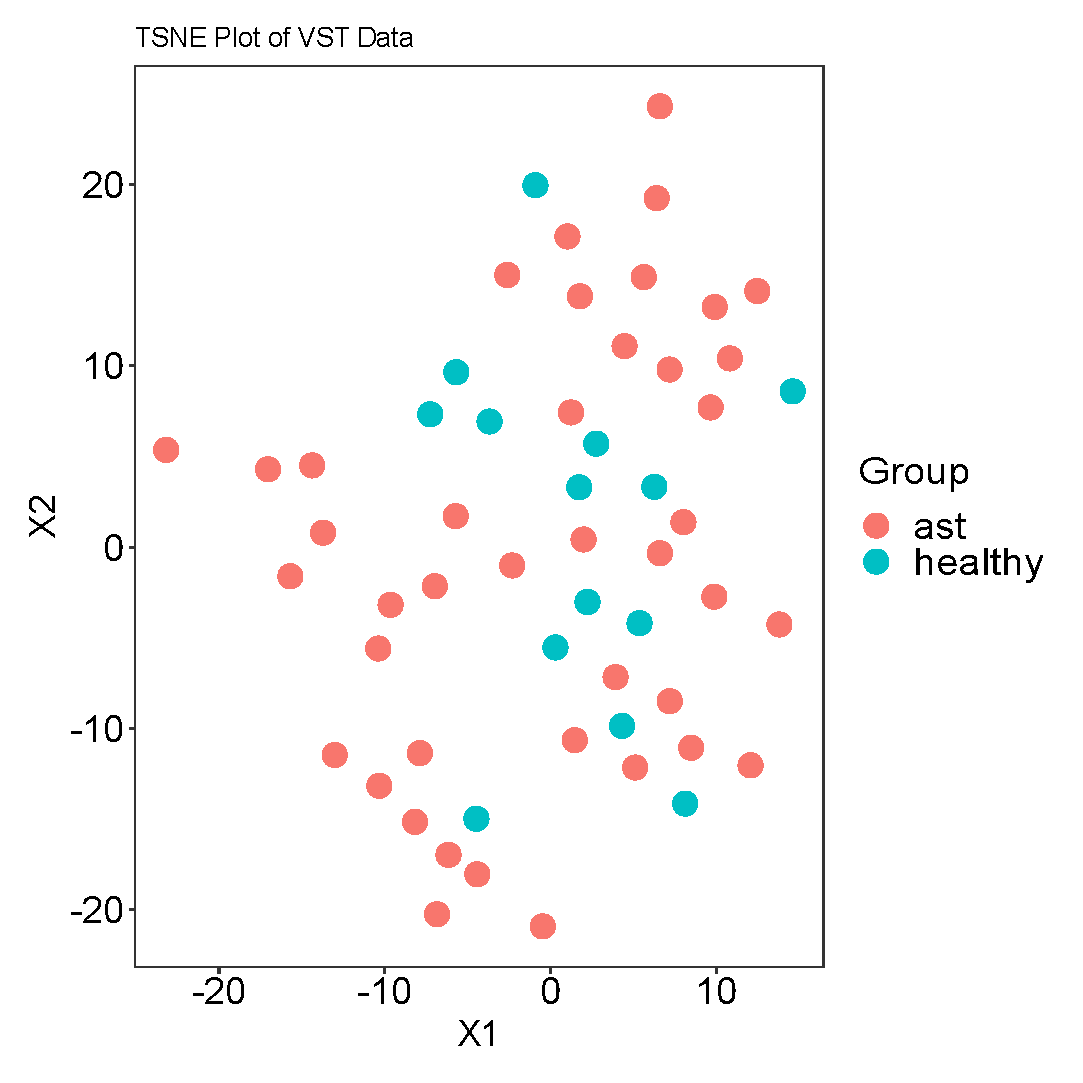
\includegraphics[scale=0.4]{plots/assn2/tsne_plot.eps}
    \caption{t-SNE Plot of DeSeq Data}
    \label{fig:tsne}
\end{figure}
\begin{figure}[h!]
    \centering
    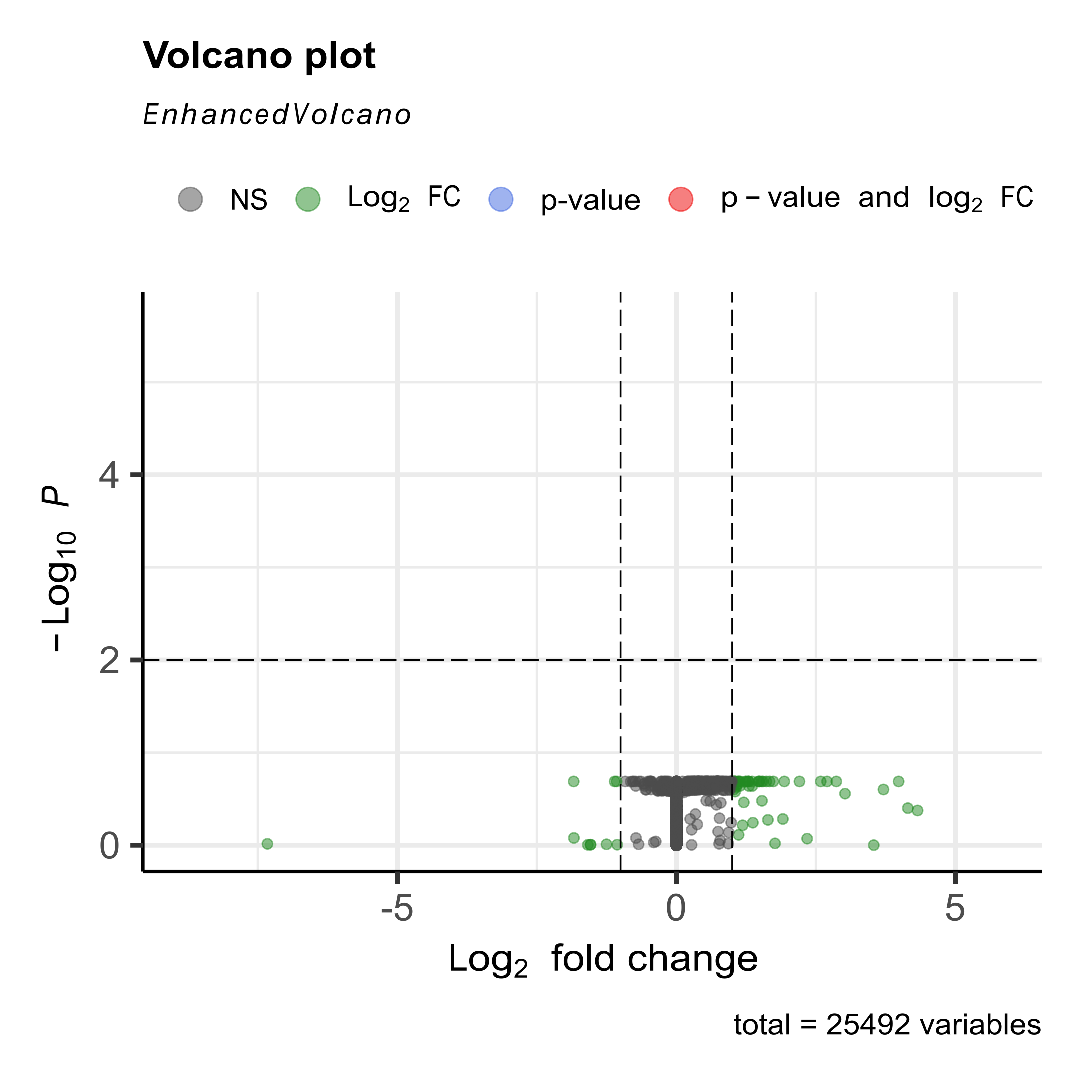
\includegraphics[scale=0.5]{plots/assn2/volcano_plot.eps}
    \caption{Volcano Plot showing statistical significance and log-Fold Change.}
    \label{fig:volcano}
\end{figure}
\begin{sidewaysfigure}[h!]
    \centering
    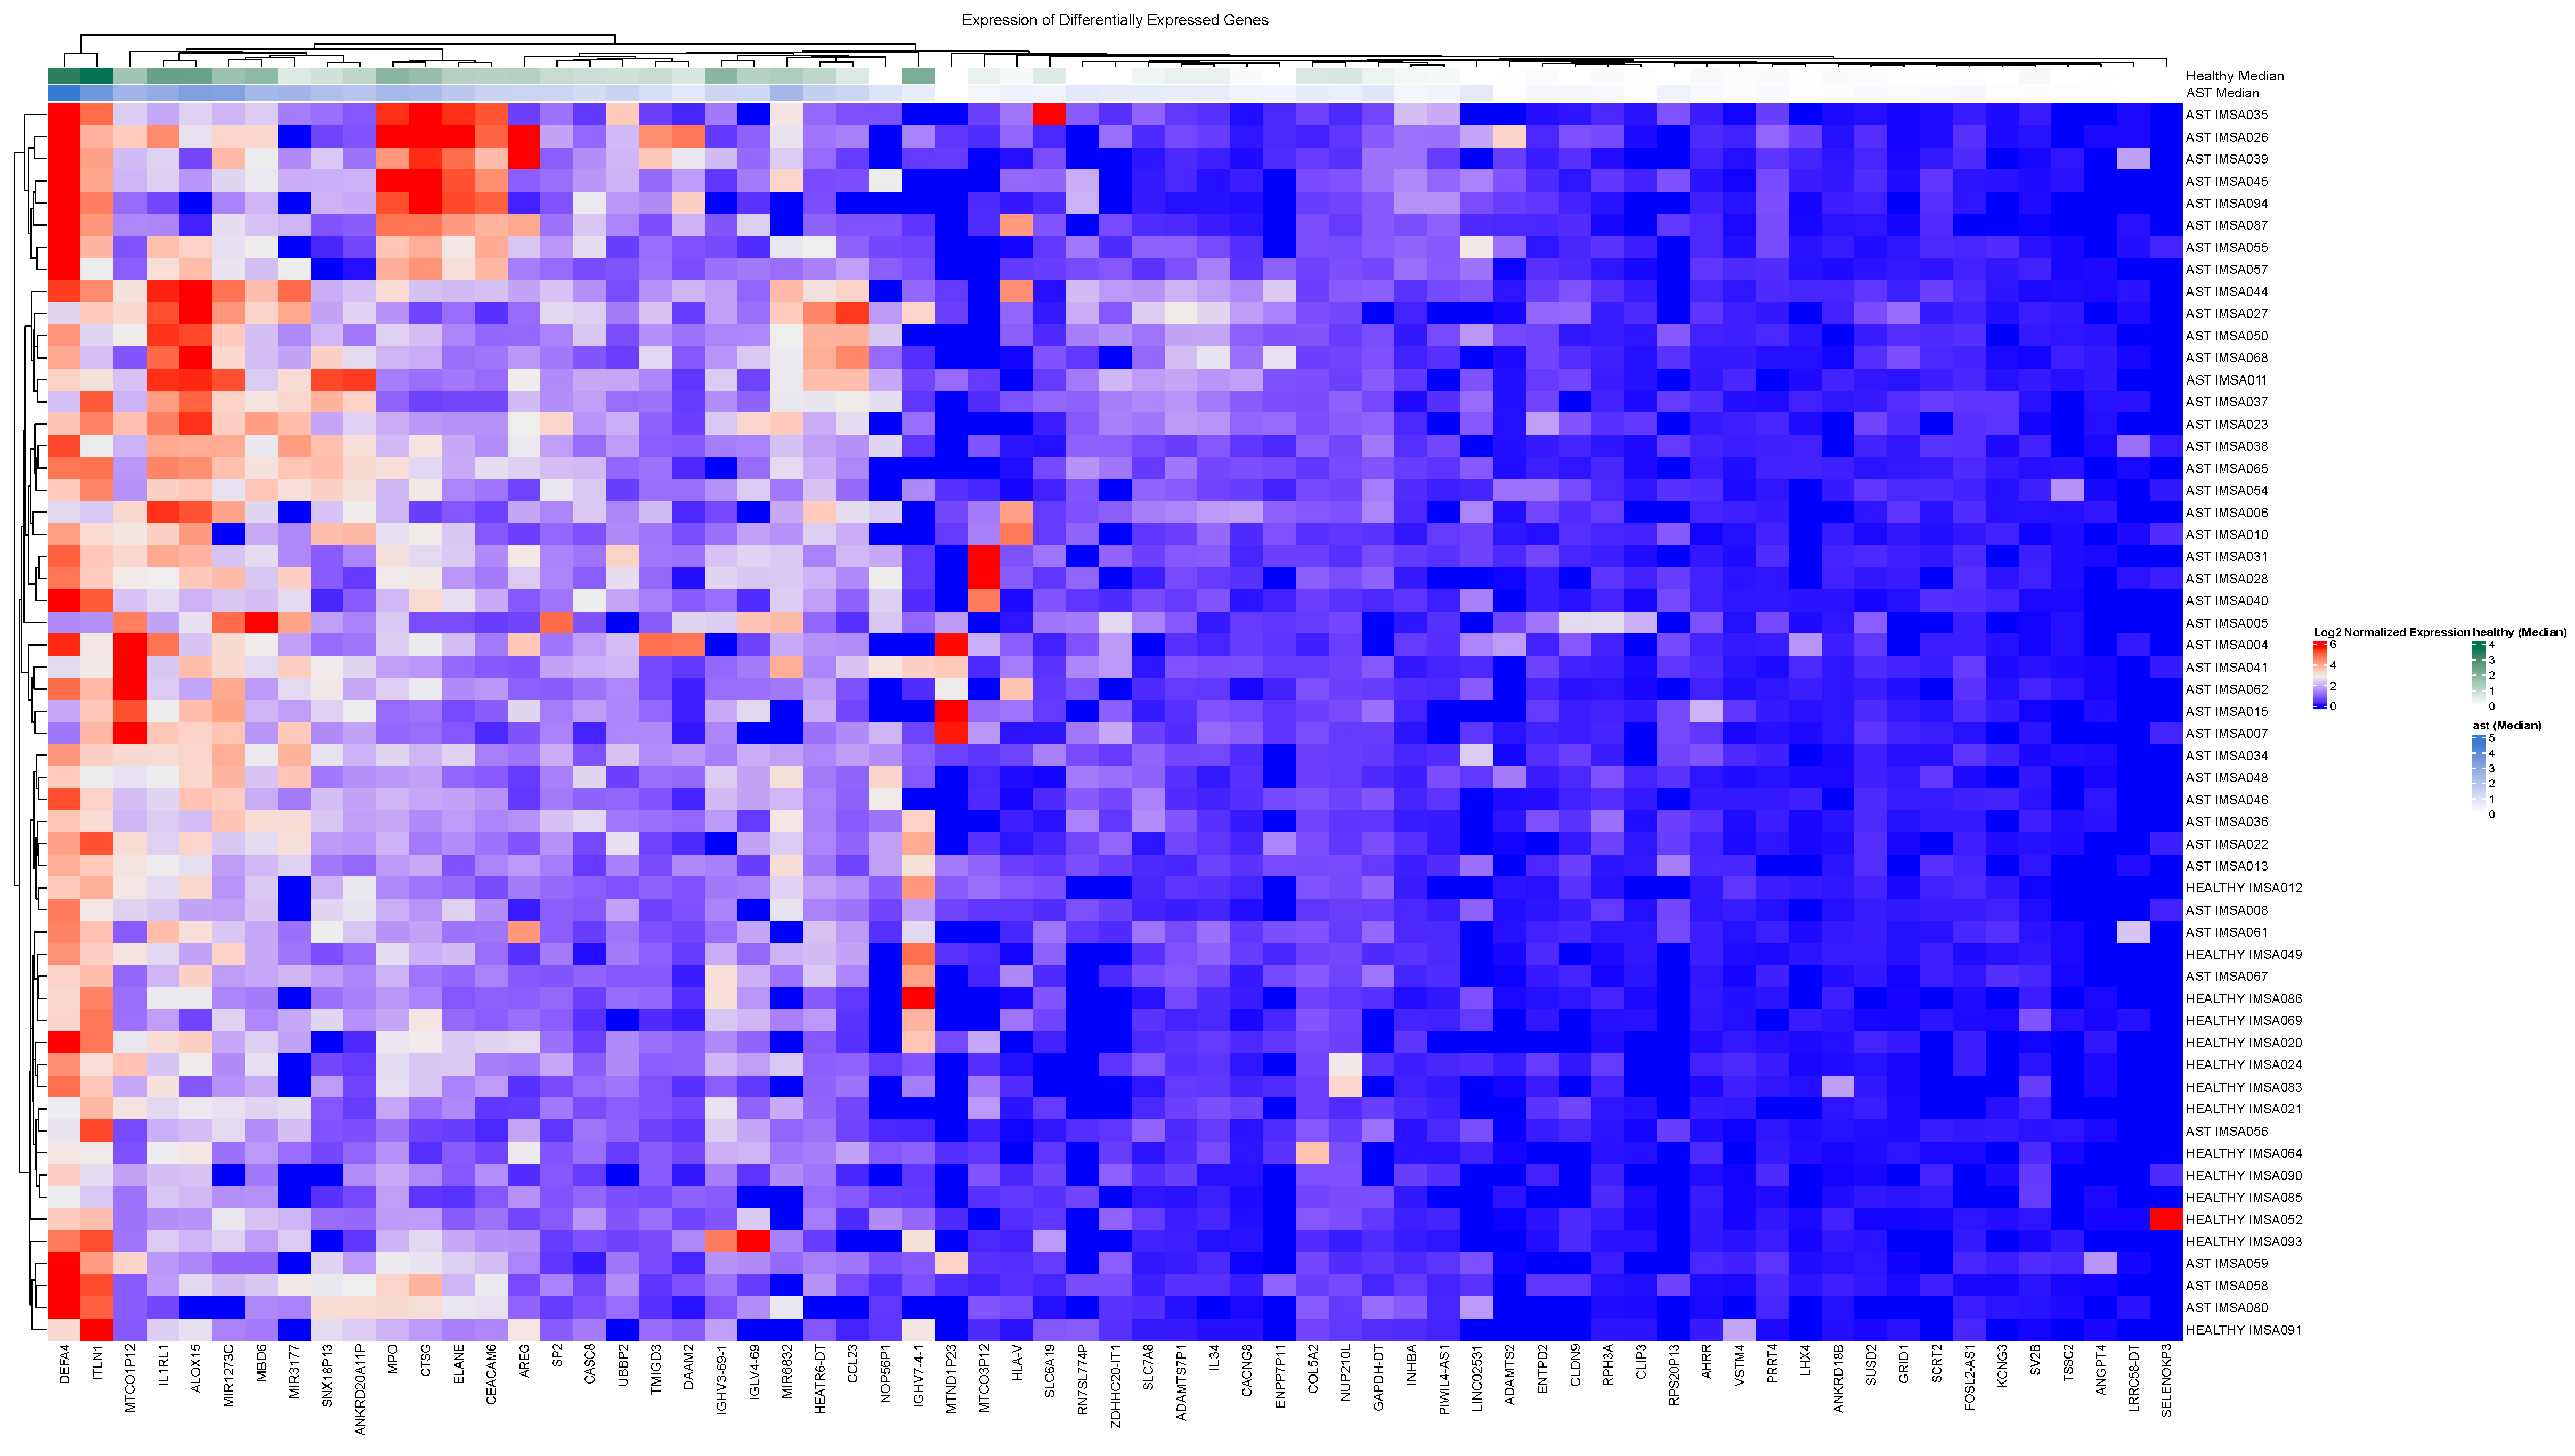
\includegraphics[scale=0.2]{plots/assn2/heatmap_plot.eps}
    \caption{Heatmap showing the expression of genes with highest logFold Change}
    \label{fig:heatmap}
\end{sidewaysfigure}
\clearpage
Cluster analysis corroborates the results from other tests regarding statistical significance, while showing that analyzing different amounts of genes leads to varying effectiveness of confounding variables. Neither \texttt{ConsensusClusterPlus} with Hierarchical clustering, PAM, nor KMeans show significant statistical dependence with the experimental condition, while showing statistical dependence among each other. (\betterref{tab:cluster}) Beyond this, while two methods had the same optimal number of clusters as the condition (\betterref{fig:factoextra}), \betterref{fig:consensus} shows that ConsensusClusterPlus had significantly more, at 10 clusters. In addition, all methods show differences in sample clustering depending on the amount of genes used for the cluster analysis (Figs.~\ref{fig:ccpalluvial}, \ref{fig:kmeansalluvial} and \ref{fig:pamalluvial}), which suggest that questions regarding the expression of specific sets of genes may result in varied conclusions, with different confounding variables. \\
\\\\
\begin{table}[H]
    \centering
    \resizebox{\textwidth}{!}{\begin{tabular}{@{}lllllll@{}}
    \toprule
     & ConditionPAM & ConditionKMeans & ConditionCCP & PAMKMeans & PAMCCP & KMeansCCP \\
    \midrule
    p-value & 0.03250944 & 0.6325851 & 0.2205631 & 1.448363e-07 & 1.593233e-06 & 3.420940e-06 \\
    p-adj & 0.09752833 & 0.6325851 & 0.4411262 & 8.690175e-07 & 7.966164e-06 & 1.368376e-05 \\
\bottomrule
    \end{tabular}}
    \caption{Statistical Independence of Clustering Algorithms when compared amongst themselves and the experimental condition.}
    \label{tab:cluster}
\end{table}
\begin{figure}[h!]
    \centering
    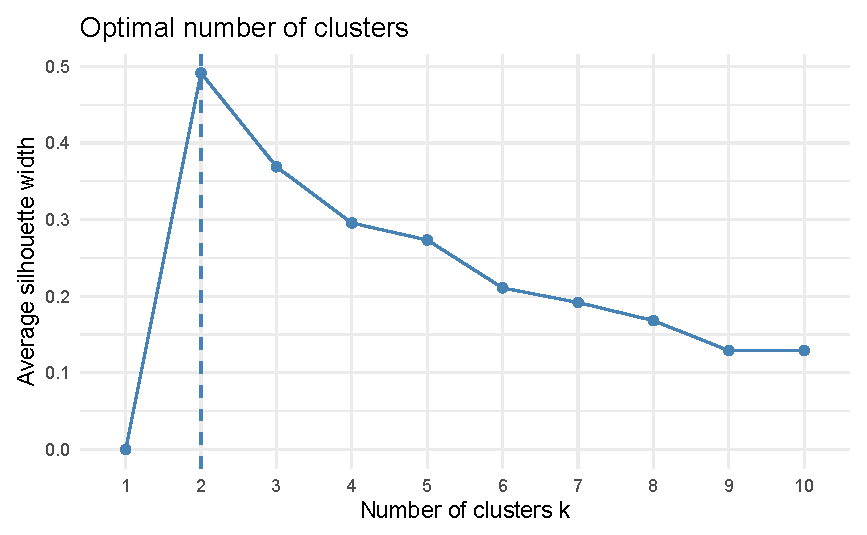
\includegraphics[scale=0.6]{plots/assn3/PAM/OptimalKValues/fivek_optimalclusters.eps}
    \caption{Optimal Amount of Clusters as determined by \texttt{factoextra} \cite{factoextra}}
    \label{fig:factoextra}
\end{figure}
\begin{figure}[h!]
    \centering
    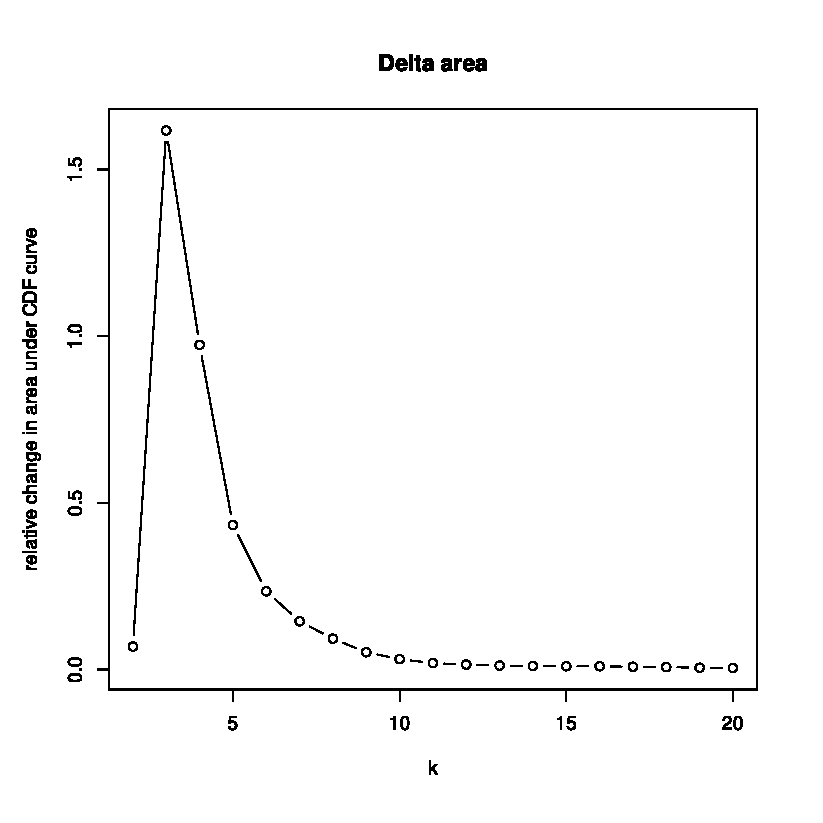
\includegraphics[scale=0.7]{plots/assn3/CCP/Top5000Genes/consensus022.eps}
    \caption{Additional variability accounted for by additional clusters}
    \label{fig:consensus}
\end{figure}
\begin{figure}[h]
    \centering
    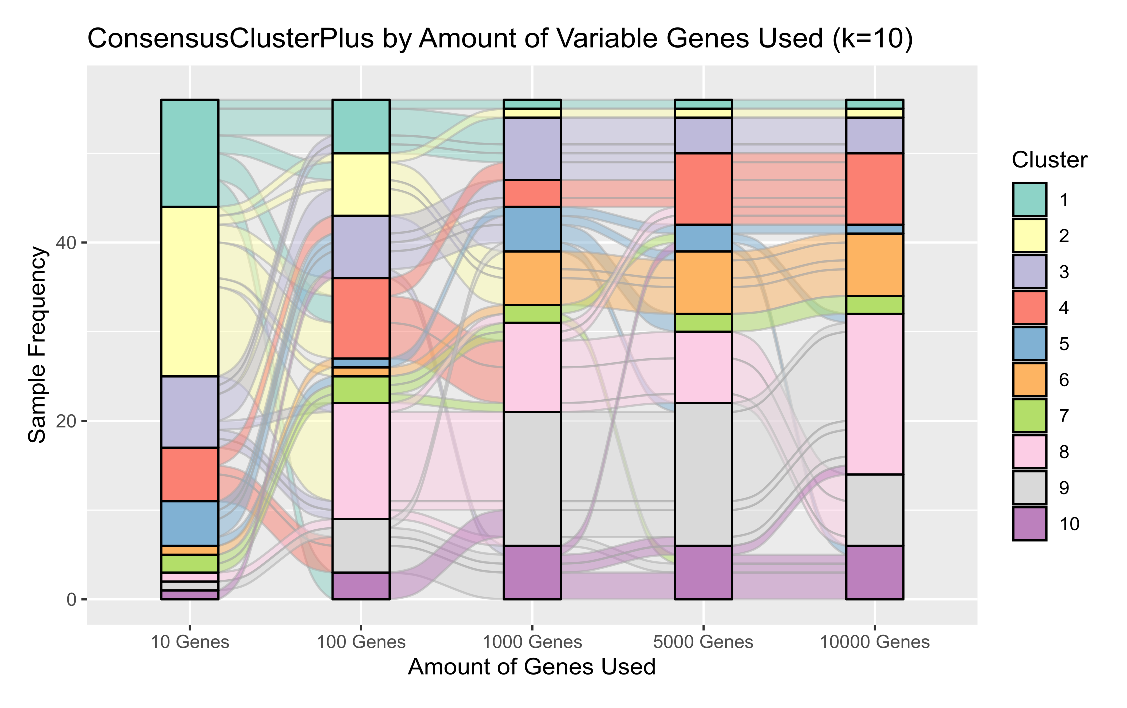
\includegraphics[scale=0.6]{plots/assn3/Alluvials/Alluvial_CCC.eps}
    \caption{Differences in \texttt{ConsensusClusterPlus} sample clusters when more genes are used in cluster analysis.}
    \label{fig:ccpalluvial}
\end{figure}
\begin{figure}[h]
    \centering
    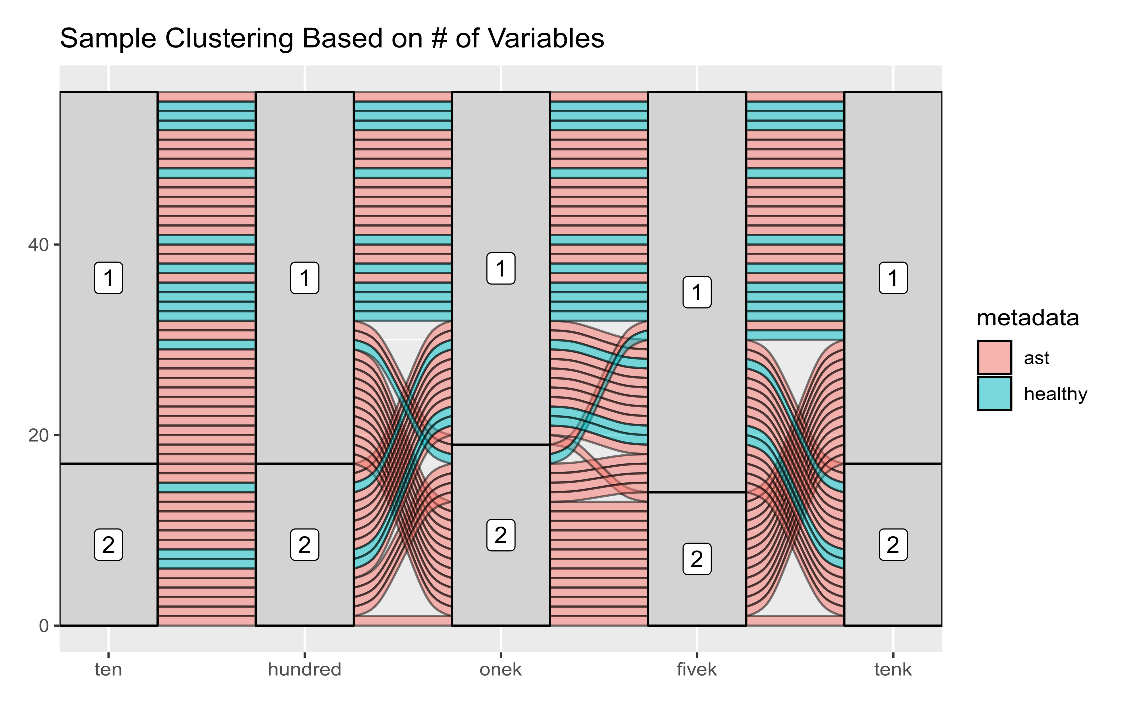
\includegraphics[scale=0.6]{plots/assn3/Alluvials/Alluvial_PAM.eps}
    \caption{Differences in PAM sample clusters when more genes are used in cluster analysis.}
    \label{fig:pamalluvial}
\end{figure}
\begin{figure}[h]
    \centering
    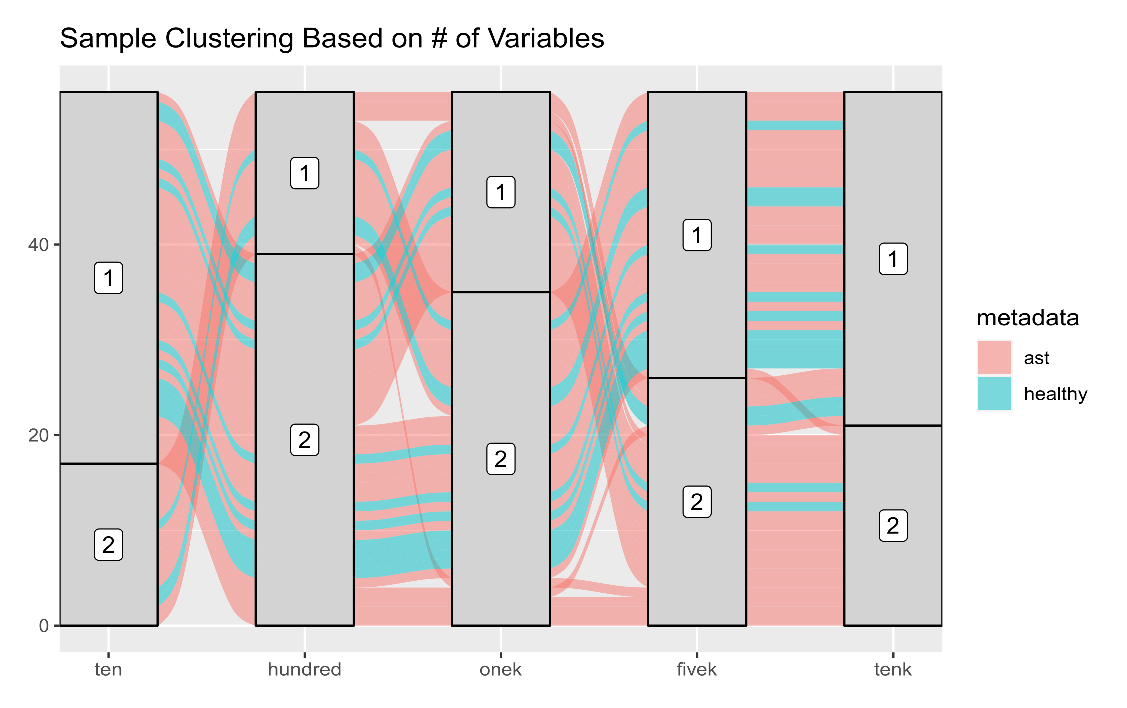
\includegraphics[scale=0.6]{plots/assn3/Alluvials/Alluvial_KMeans.eps}
    \caption{Differences in KMeans sample clusters when more genes are used in cluster analysis.}
    \label{fig:kmeansalluvial}
\end{figure}

\clearpage
Finally, while independent analysis of the dataset reveals no significant differences in expression, enrichment suggests certain processes and components with which the gene expressions found within the dataset correlate. Enriching with the GO:Biological Processes database \cite{ashburner2000gene} (\betterref{fig:bp}) included biological processes relating to different responses to fungus and stimulus in general, while the GO:Cellular Components and REACTOME database \cite{ashburner2000gene, fabregat2018reactome} (Figs.~\ref{fig:cc} and \ref{fig:reac}) show correlation with cellular components involved in the lysosome, azurophilic granules, other antimicrobial peptides and extracellular space. While some of these tasks are the primary purposes of PBMCs, their p-values suggest that these pathways could be an important area of further research. However, analysis of this dataset did not find a statistically significant difference in gene expression between patients with or without asthma.
\begin{figure}[h]
    \centering
    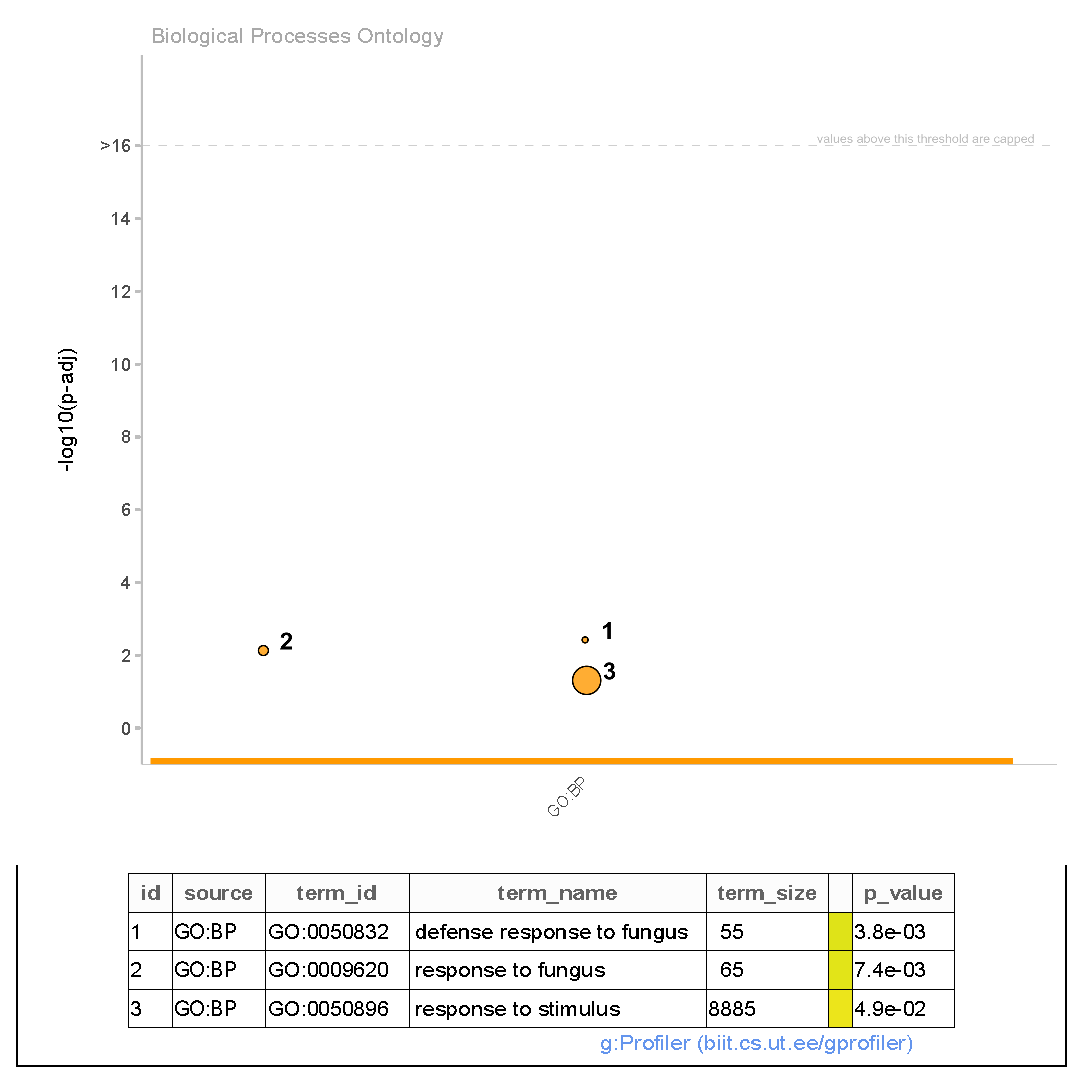
\includegraphics[scale=0.45]{plots/assn2/bp_onto_plot.eps}
    \caption{\texttt{g:Profiler} enrichment analysis of differentially expressed genes using the GO Biological Processes Database}
    \label{fig:bp}
\end{figure}
\begin{figure}[h]
    \centering
    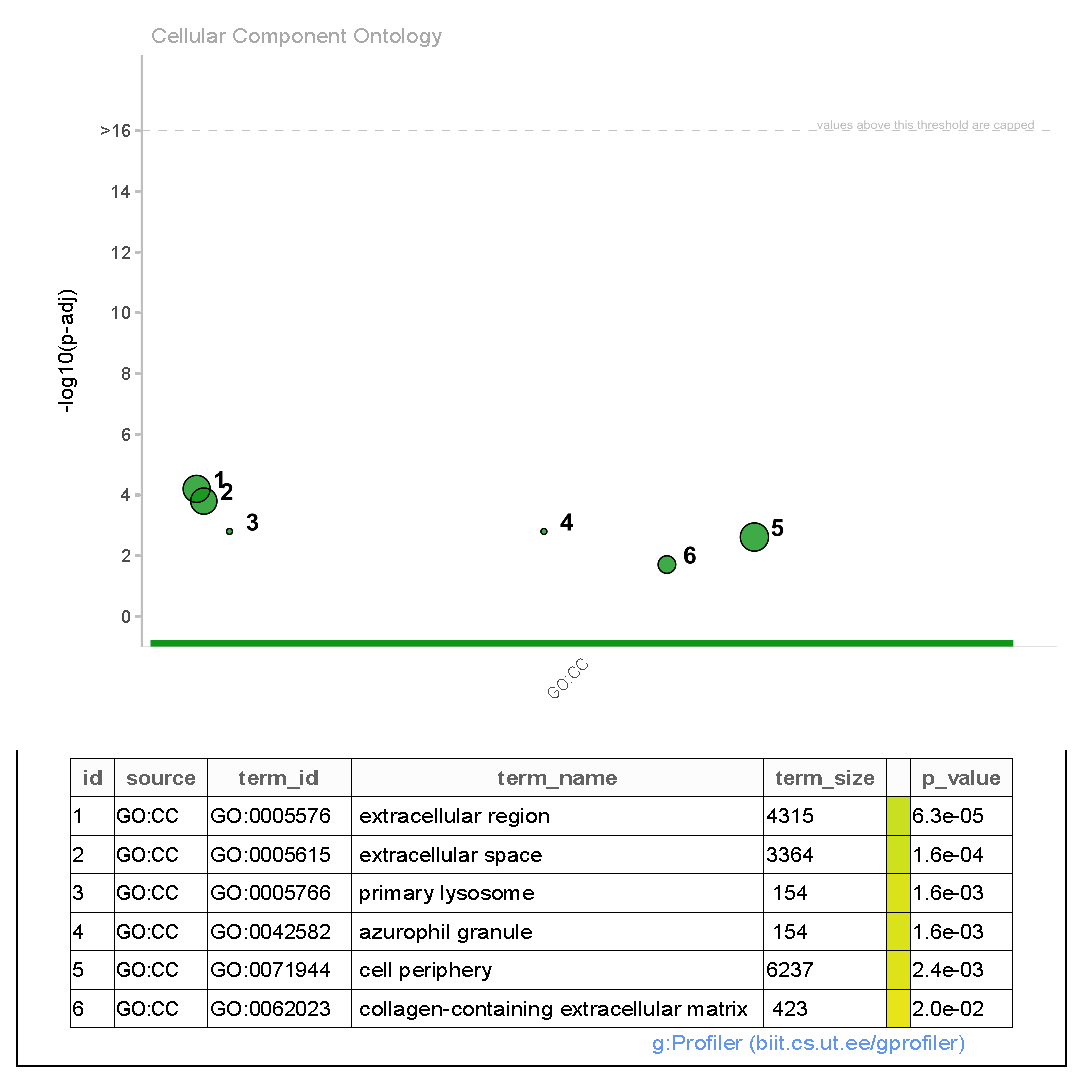
\includegraphics[scale=0.45]{plots/assn2/cc_onto_plot.eps}
    \caption{\texttt{g:Profiler} enrichment analysis of differentially expressed genes using the GO Cellular Components Database}
    \label{fig:cc}
\end{figure}
\begin{figure}[h]
    \centering
    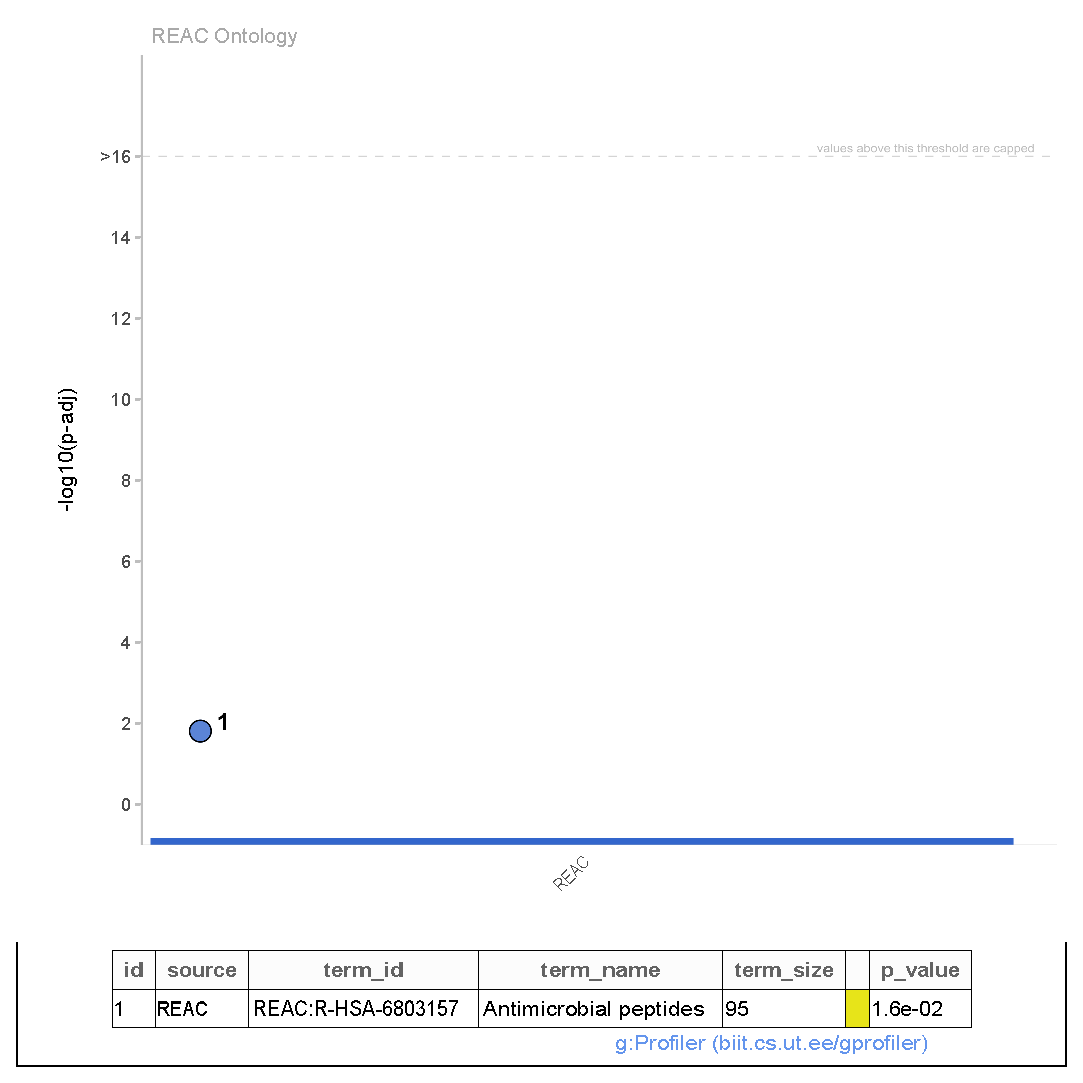
\includegraphics[scale=0.45]{plots/assn2/reac_onto_plot_special.eps}
    \caption{\texttt{g:Profiler} enrichment analysis of differentially expressed genes using the REACTOME Database}
    \label{fig:reac}
\end{figure}
\clearpage
\section{Conclusion}\label{sec4}
Overall, statistical analysis did not find a significant difference in gene expression between asthmatic and healthy patients. There were no genes whose difference in expression were statistically significant per DeSeq analysis. Clustering analysis also showed that much of the variance in gene expression is not directly related to the experimental condition. The likely reason that the analysis of the data did not provide meaningful results was the limited sample size. While there were many genes in the data set, samples were taken from only 56 different patients, leading to low statistical power. Analysis of gene expression of a larger sample size will yield more meaningful results. Other problems with our study include the difficulty in studying a disease as variable as asthma. As such, we expect a high level of variability within our experimental group, making analysis difficult. Finally, our dataset may suffer from selection biases, as it comes from a single lab in Massachusetts. As such, results may not be applicable to other parts of the world, especially with asthma often being related to environmental factors. \\
However, the analysis still showed interesting paths for further investigation. Enrichment analysis identified genes that correspond to biological processes involving response to stimulus, and response to fungi. These biological processes and cellular components have previously been correlated with asthma \cite{Holgate2012-et, Denning2006-jd}, and this analysis may point to specific genes and pathways which cause these correlations to occur. These results from enrichment analysis suggest the need for further investigation, which may uncover specific pathways that lead to an asthmatic response to immune stimuli and fungi. However with the current data set, no significant difference or relationship between the gene expression of healthy and asthmatic patients’ PBMC cells could be found. Due to the limitations on our dataset, we would need to generate additional experimentation on a larger sample of patients in order to possibly identify SSDEGs and further investigate any link between the expression of the immune cells and asthma acquisition in a setting where statistical significance can be supported.


\begin{appendices}


%%=============================================%%
%% For submissions to Nature Portfolio Journals %%
%% please use the heading ``Extended Data''.   %%
%%=============================================%%

%%=============================================================%%
%% Sample for another appendix section			       %%
%%=============================================================%%

%% \section{Example of another appendix section}\label{secA2}%
%% Appendices may be used for helpful, supporting or essential material that would otherwise 
%% clutter, break up or be distracting to the text. Appendices can consist of sections, figures, 
%% tables and equations etc.

\end{appendices}

%%===========================================================================================%%
%% If you are submitting to one of the Nature Portfolio journals, using the eJP submission   %%
%% system, please include the references within the manuscript file itself. You may do this  %%
%% by copying the reference list from your .bbl file, paste it into the main manuscript .tex %%
%% file, and delete the associated \verb+\bibliography+ commands.                            %%
%%===========================================================================================%%
\pagebreak
\bibliography{sn-bibliography}% common bib file
%% if required, the content of .bbl file can be included here once bbl is generated
%%\input sn-article.bbl

%% Default %%
%%\input sn-sample-bib.tex%

\end{document}
